\documentclass[10pt]{beamer}

\usepackage[ngerman]{babel}
\usepackage{amsmath}
\usepackage{bbm}
\usepackage{tikz}

\usepackage{tabularx}
\usepackage{graphicx}
\usepackage{subcaption}
\usepackage{url}
\usepackage{eurosym}
\usepackage{listings}
\usepackage{datetime}
\usepackage[style=authoryear, backend=biber]{biblatex}

\usepackage{epstopdf}

\usepackage{multirow}
\usepackage{colortbl}
\usepackage{booktabs}

\newif\ifzihbackground
\zihbackgroundtrue
%\zihbackgroundfalse

% Yes, this is dirty
\newcommand\zihmaketitle{
	\definecolor{white}{gray}{1.00}%
	\setbeamercolor{normaltext}{bg=darkblue}%
	\setbeamertemplate{headline}{%
		\vskip6.15mm\color{white}\setlength{\arrayrulewidth}{0.3pt}%
		\begin{tabular*}{\paperwidth}[b]{l@{\extracolsep\fill}}%
			\hspace*{3.0mm}\color{white}%
			
\includegraphics[height=7.81mm]{theme/logo/tu_logo_black}\\[1.2mm]%
			\hline\hspace*{11.76mm}\rule[-0.8mm]{0pt}{2.47mm}%
			\def\@@dummyComma{}\rule{0pt}{5.8pt}%
			\insertinstitute \\%
			\hline%
		\end{tabular*}%
		\hspace{-\paperwidth}%
	}%
    \ifzihbackground
      \setbeamertemplate{footline}{}
      \setbeamertemplate{background}{
\includegraphics[height=\paperheight,width=\paperwidth]{theme/logo/bg}}
      \else
      \setbeamertemplate{footline}{
          \parbox[t][22mm]{\paperwidth}{
              \vspace*{-8.18mm}
              \rule
              {98.6mm}{0pt}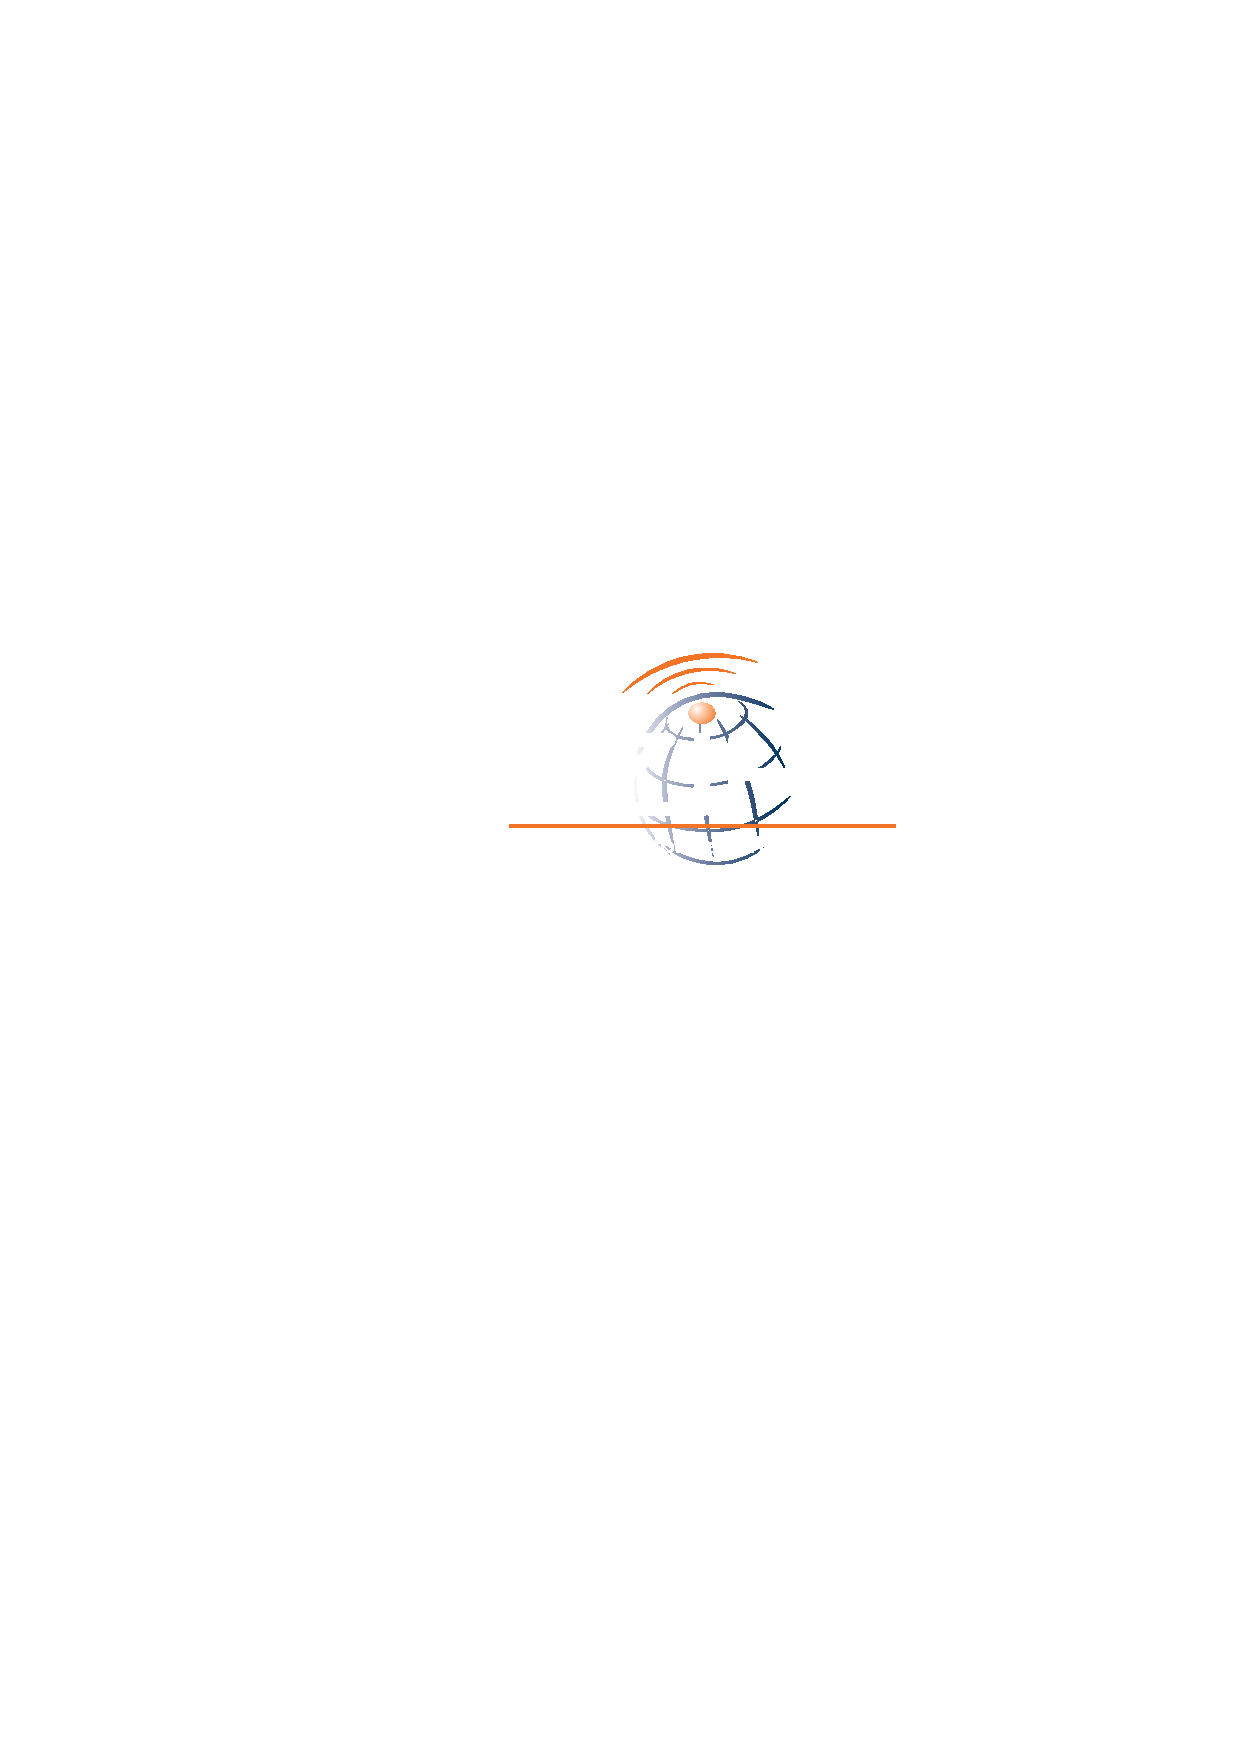
\includegraphics[height=15mm]{theme/logo/zih_logo_white}

          }
      }
    \fi%
   \frame{\titlepage}
    % Kopf-/Fusszeilen fuer restliche Folien
    \setbeamercolor{normal text}{bg=white}
    \setbeamertemplate{background}{}
    \setbeamertemplate{headline}[zih01 theme]
    \setbeamertemplate{footline}[zih01 theme]
}

\usetheme{Dresden}
%\useoutertheme{theme/zih01}
%\useinnertheme{theme/zih01}
\usepackage{theme/beamerouterthemezih01}
\usepackage{theme/beamerinnerthemezih01}

%\useinnertheme{rounded}
\definecolor{darkblue}{rgb}{0.04, 0.16, 0.32}
% font color for headlines etc.
\setbeamercolor*{structure}{fg=darkblue,bg=white}
% disable navigation symbols
\setbeamertemplate{navigation symbols}{}
% can't remember what this is good for
\setbeamercovered{transparent}

% reduce margin size
\setbeamersize{text margin left=0.7cm}
\setbeamersize{text margin right=0.7cm}
%
% Outer Color Theme "whale" sorgt f?r strenge farbliche Trennen zwischen Zierrat
% und dem eigentlichen Inhalt. Ein dunkler Hintergrund f?r den Folientitel wirkt
% aber zu aufdringlich.
%
\usecolortheme{orchid}
%\setbeamercolor{titlelike}{parent=structure}

%
% Inner Color Theme "orchid" sorgt f?r farblich abgesetzt Bl?cke (Definitionen,
% S?tze, Beispiele, Beweise, ...).
%
%\usecolortheme{orchid}

%zum drucken
%\usepackage{pgfpages}
%\pgfpagesuselayout{resize to}[a4paper,border shrink=5mm,port]
%\pgfpagesuselayout{4 on 1}[a4paper,border shrink=3mm, landscape]

%%%%%%%%%%%%%%%%%%%%%%%%%%%%

\definecolor{LightGray}		{gray}{0.9}
\definecolor{Gray}		{gray}{0.5}
\definecolor{DarkGray}     	{gray}{0.2}
\definecolor{listinggray} 	{gray}{0.96}
\definecolor{DarkGreen}     	{rgb}{0.0,0.6,0.0}
\definecolor{DarkRed}     	{rgb}{0.6,0.0,0.0}
\definecolor{DarkBlue}     	{rgb}{0.0,0.0,0.6}
\definecolor{DarkCyan}     	{rgb}{0.7,0.7,0.2}
\definecolor{DarkDarkGreen}	{rgb}{0.0,0.4,0.0}

\lstset{language=C}
\lstset{linewidth=0.99\textwidth}
%\lstset{boxpos=c}
\lstset{xleftmargin=0.03\textwidth}
%\lstset{breaklines=true}
\lstset{framexleftmargin=0.03\textwidth}
\lstset{abovecaptionskip=\smallskipamount}
\lstset{belowcaptionskip=\smallskipamount}
\lstset{basicstyle=\ttfamily\tiny}
\lstset{backgroundcolor=\color{listinggray}}
%\lstset{frameround=ffff}
%\lstset{frame=shadowbox}
%\lstset{rulesepcolor=\color{Gray}}
\lstset{numbers=left}
\lstset{numberstyle=\tiny \color{DarkGray}}
\lstset{numbersep=0.01\textwidth}
\lstset{showstringspaces=false}
%\lstset{showspaces=false}
\lstset{tabsize=4}

%% all words in the following list are printed in bold letters in a listing 
\lstset{emph={__asm__, __volatile__, return, main,},emphstyle={\bfseries\color{DarkGray}}}
\lstset{captionpos=b}

% Style für C Sourcecode
\lstdefinestyle{CA}{
        language=C,
        basicstyle=\ttfamily\scriptsize,
        keywordstyle=\ttfamily\bfseries\color{DarkBlue},
        stringstyle=\ttfamily\color{DarkRed},
        commentstyle=\ttfamily\color{DarkGreen},
        identifierstyle=\ttfamily\color{DarkCyan},
        backgroundcolor=\color{listinggray},
}

%%%%%%%%%%%%%%%%%%%%%%%%%%%%

% define blocks for flowchart
\usetikzlibrary{shapes.geometric, arrows}
\date{\today}
\institute[TI TUD]{Institut für Technische Informatik, Professur für Rechnerarchitektur -- TU Dresden}
\title[PWFRA]{Parallelisierung des Wellenfrontrekonstruktionsalgorithmus auf Multicore-Prozessoren}
%\subtitle{Zwischenpräsentation}
\author[Schenke]{Jonas~Schenke}

\DeclareCiteCommand{\citejournal}
{\usebibmacro{prenote}}
{\usebibmacro{citeindex}%
	\usebibmacro{journal}}
{\multicitedelim}
{\usebibmacro{postnote}}

\newcommand{\citeall}[1]{\citetitle{#1}, \cite{#1}, \citejournal{#1}}

\hsl{Prof. Dr. Wolfgang E. Nagel}
\betreuer{Dr. Elena-Ruxandra Cojocaru, Dr. Michael Bussmann, Matthias Werner}
\email{jonas.schenke@tu-dresden.de}
\newdate{date}{16}{04}{2017}
\date{\displaydate{date}}

\addbibresource{res/Referenzen.bib}

% Zu jedem Abschnitt Gliederung zeigen
\AtBeginSection[]
{
  \begin{frame}<beamer>{Gliederung}
    \tableofcontents[currentsection]
  \end{frame}
}

% auch bei subsections gliederung?
%\AtBeginSubsection[]
%{
%  \begin{frame}<beamer>{Gliederung}
%    \tableofcontents[currentsection,currentsubsection]
%  \end{frame}
%}

% bei sehr vielen sections, mehrspaltig
%\begin{frame}[shrink]
%\frametitle{Gliederung}
%\begin{multicols}{2}
%	\tableofcontents
%\end{multicols}
%\end{frame}

% alle Aufzaehlungen schrittweise zeigen
%\beamerdefaultoverlayspecification{<+->}

\begin{document}

\zihmaketitle

\begin{frame}{Aufgabenstellung}
\frametitle{Aufgabenstellung}
	\begin{itemize}
		\item Evaluierung und Performance-Analyse des derzeit fast durchgängig seriellen Wellenfrontrekonstruktionsalgorithmus
		\item Parallelisierung der kritischen Pfade für Mehrkernarchitekturen
		\item Performance-Messungen der parallelen Implementation
		\item Auswertung sowie Validierung der Ergebnisse
	\end{itemize}
\end{frame}

\begin{frame}{Gliederung}
  \setcounter{tocdepth}{1} 
  \tableofcontents
  % Die Option [pausesections] koennte nuetzlich sein.
\end{frame}



% im text korrekturen anzeigen
\newcommand{\correctme}[1]{\textcolor{red}{#1}}

% korrekturen ueber mehrere absaetze
\newenvironment{correctmore}{\color{red}}{\color{black}}

\lstset{
	backgroundcolor=\color{white},
	commentstyle=\color{green},
	frame=single,
	keywordstyle=\color{blue},
	breaklines=true,
	numbers=left,
	numbersep=5pt,
	tabsize=4,
	basicstyle=\footnotesize,
}

%TODO: 0. Einleitung --> Motivation % Hintegrund		1 -.    
%TODO: 1. Disclaimer									1  | 10 
%TODO: 2. Der Wellenfrontrekonstruktionsalgorithmus		4  |    
%TODO: 3. Performance									4 -'    
%TODO: 4. Optimierung									1 -.    
%TODO: 4.1 Parallelisierung								4  | 10 
%TODO: 4.2 Optimierung									5 -'    
%TODO: 5. wieder Performance							7 -.    
%TODO: 6. Ausblick										3 -' 10 

\section{Hinweise}

\begin{frame}{Hinweise}
	\begin{itemize}
		\item<2-> Teil des \textbf{Eu}ropean \textbf{C}luster of \textbf{A}dvanced \textbf{L}aser \textbf{L}ight Sources (EUCALL)-Projektes
		\rightarrow Überschneidung von \textbf{U}ltra\textbf{f}ast \textbf{D}ata \textbf{Ac}quisition (UFDAC; WP5) und \textbf{Pu}lse \textbf{C}haracterisation and \textbf{C}ontrol (PUCCA; WP7)
		\item<3-> Zusammenarbeit des \textbf{H}elmholtz-\textbf{Z}entrum \textbf{D}resden-\textbf{R}ossendorf e.V. (HZDR) und \textbf{E}uropean \textbf{S}ynchrotron \textbf{R}adiation \textbf{F}acillity (ESRF)
		\item<4-> \textbf{Algorithmus:} Sébastien Bérujon
		\item<5-> \textbf{Code:} Elena-Ruxandra Cojocaru
	\end{itemize}
\end{frame}

\begin{frame}{Hinweise}
	\textbf{Daten:} Beamline BM05, ESRF, Grenoble, Frankreich
	\begin{tabularx}{\textwidth}{@{} XXX @{}}
		\toprule
		& \textbf{Experiment 6} & \textbf{Lenses} \\
		\hline
		Aufnahmedatum & Ruxandra Cojocaru, Sébastien Bérujon, Eric Ziegler & Thomas Rothand, Raymond Barett, Sébastien Bérujon, Rafael Celeste \\
		Aufgenommen von & 24. September 2017 & 10. April 2017 \\
		\bottomrule
	\end{tabularx}
\end{frame}
\section{Evaluierung des Wellenfrontrekonstruktionsalgorithmus}

\subsection{Überblick}
\begin{frame}{Versuchsaufbau}
	\begin{tikzpicture}
		\node at (0,0) {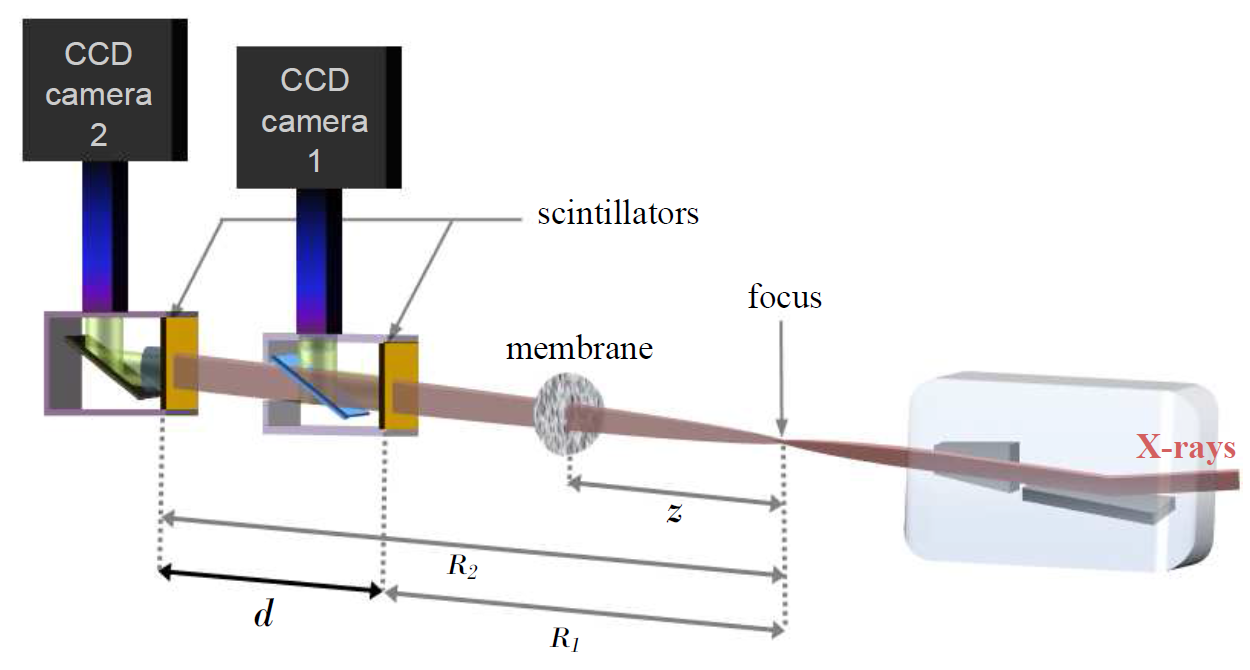
\includegraphics[width=0.98\linewidth]{./img/Versuchsaufbau.png}};
		\only<2>{\draw[red, very thick] (2.4, -2.2) rectangle (5.5, -0.2);}
		\only<3>{\draw[red, very thick] (1.2, -1.2) rectangle (1.6, -0.8);}
		\only<4>{\draw[red, very thick] (-1.1, -1.4) rectangle (0.3, 0);}
		
		\only<5>{\draw[red, very thick] (-5.5, 2.9) rectangle (-1.7, -1);}
		\only<6>{\draw[red, very thick] (-4.3, -2.7) rectangle (-2.1, -2);}
		\only<7>{\draw[red, very thick] (-3.3, -1) rectangle (-1.7, 0.1);}
		
		\only<8>{\draw[red, very thick] (-3.6, 1.2) rectangle (-1.9, 2.7);}
		\only<8>{\node at (3.4,0.8) {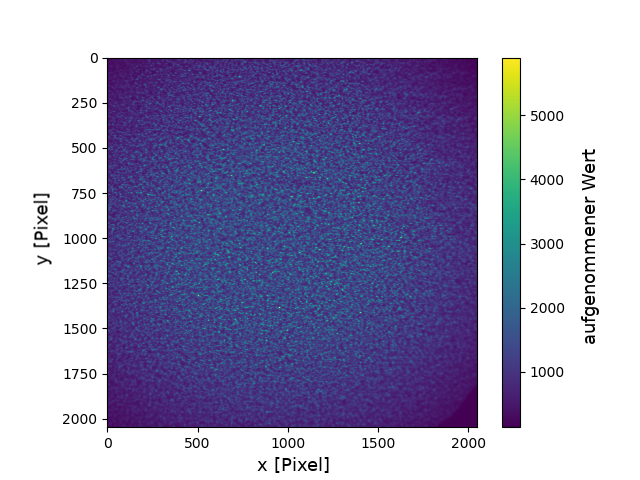
\includegraphics[width=0.5\linewidth]{img/ref_start0001_1-10}};}
		\only<8>{\draw[red, very thick] (0.7, 2.8) rectangle (6.0, -1.33);}
		\only<8>{\draw[red, very thick] (0.7, 2.8) -- (-1.9, 2.7);}
		\only<8>{\draw[red, very thick] (0.7, -1.33) -- (-1.9, 1.2);}
		
		\only<9>{\draw[red, very thick] (-5.3, -0.8) rectangle (-3.7, 0.3);}
		\only<10>{\draw[red, very thick] (-5.5, 1.5) rectangle (-3.8, 2.9);}
		
		\only<10>{\node at (3.4,0.8) {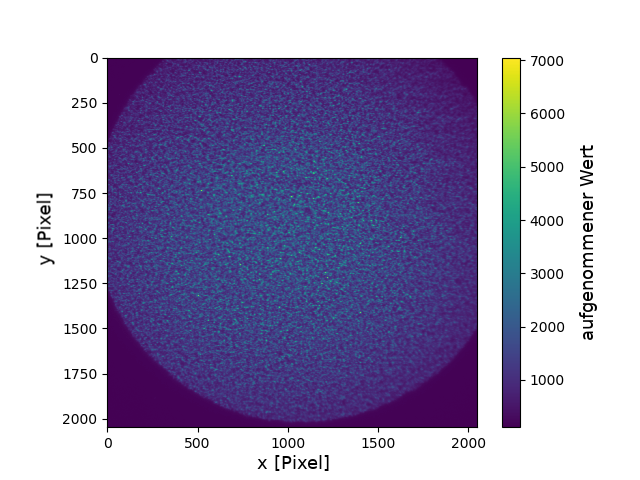
\includegraphics[width=0.5\linewidth]{img/E10001}};}
		\only<10>{\draw[red, very thick] (0.7, 2.8) rectangle (6.0, -1.33);}
		\only<10>{\draw[red, very thick] (0.7, 2.8) -- (-3.8, 2.9);}
		\only<10>{\draw[red, very thick] (0.7, -1.33) -- (-3.8, 1.5);}
	\end{tikzpicture}
	\nocite{Ber12}
	\nocite{Ber13}
	\nocite{Ber15}
	{\scriptsize \citeall{Ber15}}
\end{frame}

\begin{frame}{Überblick}
	\textbf{Hauptroutine:} 
	\begin{itemize}
		\item Korrigieren von Kamerafehlern
		\item Ablenkung nachverfolgen
		\item Wellenfront rekonstruieren
	\end{itemize}
\end{frame}

\begin{frame}{Hauptroutine}
	\only<1>{\vspace{-0.37cm}}
	\begin{tikzpicture}
		\node at (-5,0.6) {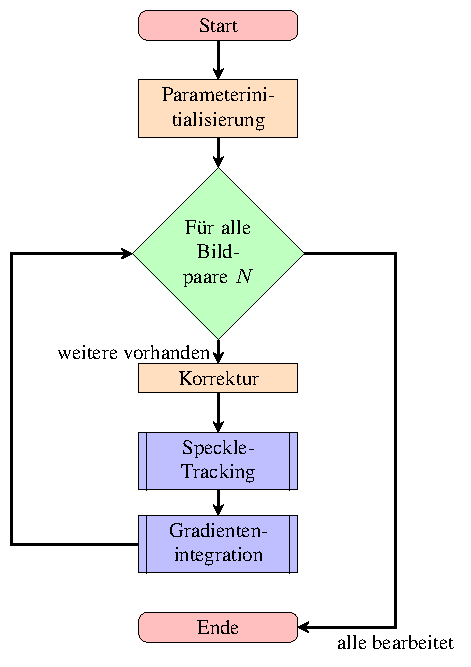
\includegraphics[width=0.4\linewidth]{pdf/graph_main}};
		\only<2-4>{\node at (-1,0) {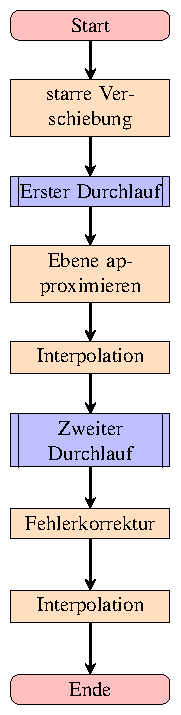
\includegraphics[width=0.17\linewidth]{pdf/graph_speckle}}};
		
		\only<2>{\draw[red, very thick] (-6.0, -1.0) rectangle (-4.3, -0.3)};
		\only<2>{\draw[red, very thick] (-4.3, -0.3) -- (-2, 3.8)};
		\only<2>{\draw[red, very thick] (-4.3, -1.0) -- (-2, -3.8)};
		\only<2>{\draw[red, very thick] (-2, -3.8) rectangle (0.0, 3.8)};
		
		\only<3-4>{\draw[red!25, very thick] (-6.0, -1.0) rectangle (-4.3, -0.3)};
		\only<3-4>{\draw[red!25, very thick] (-4.3, -0.3) -- (-2, 3.8)};
		\only<3-4>{\draw[red!25, very thick] (-4.3, -1.0) -- (-2, -3.8)};
		\only<3-4>{\draw[red!25, very thick] (-2, -3.8) rectangle (0.0, 3.8)};
		
		\only<3>{\draw[red, very thick] (-1.95, 1.5) rectangle (-0.0, 2.05)};
		\only<3>{\node at (2,0) {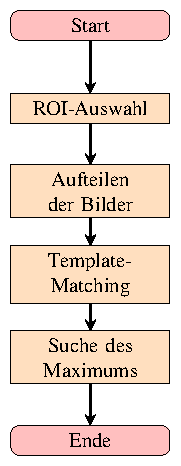
\includegraphics[width=0.17\linewidth]{pdf/graph_first_pass}}};
		\only<3>{\draw[red, very thick] (0.0, 2.05) -- (1, 2.5)};
		\only<3>{\draw[red, very thick] (0.0, 1.5) -- (1, -2.5)};
		\only<3>{\draw[red, very thick] (1.0, -2.5) rectangle (3.1, 2.5)};
		
		\only<4>{\draw[red, very thick] (-1.95, -1.25) rectangle (-0.05, -0.55)};
		\only<4>{\node at (2,0) {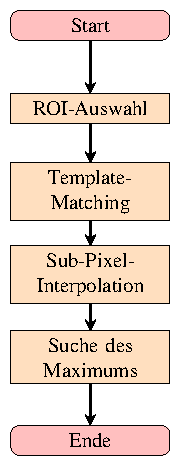
\includegraphics[width=0.17\linewidth]{pdf/graph_second_pass}}};
		\only<4>{\draw[red, very thick] (-0.05, -0.55) -- (1, 2.5)};
		\only<4>{\draw[red, very thick] (-0.05, -1.25) -- (1, -2.5)};
		\only<4>{\draw[red, very thick] (1.0, -2.5) rectangle (3.1, 2.5)};
		
		\only<5>{\draw[red, very thick] (-6.0, -1.0) rectangle (-4.3, -0.3)};
		\only<5>{\node at (1,2.2) {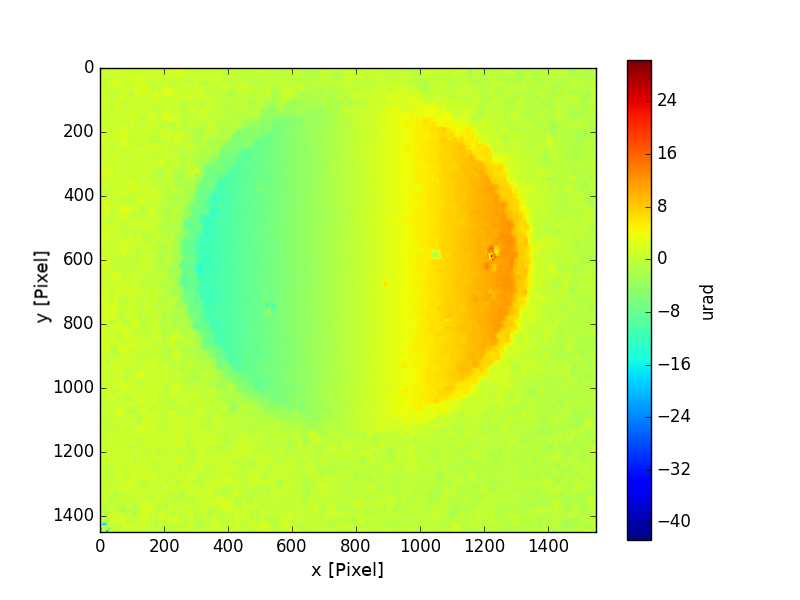
\includegraphics[width=0.38\linewidth]{img/SpeckDisH_E10001_edf_ref_start0001_1-10_edf}}};
		\only<5>{\node at (1,-1.5) {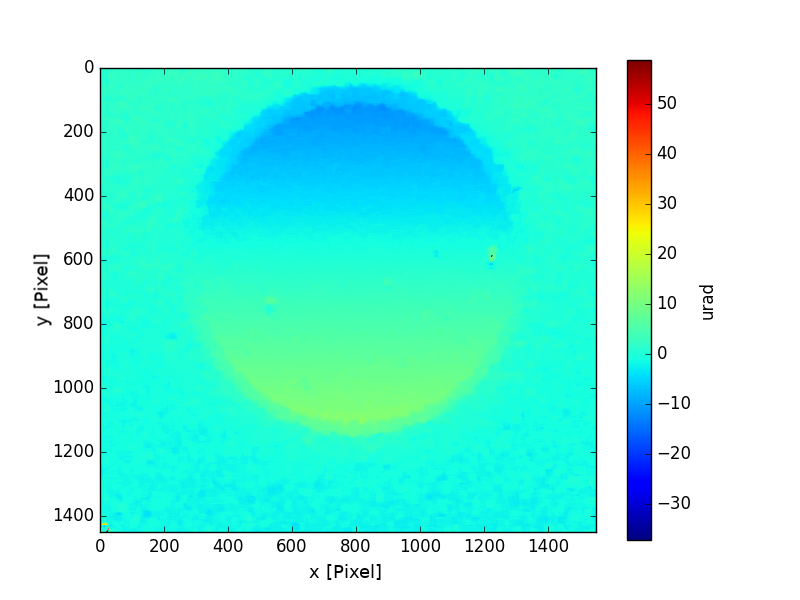
\includegraphics[width=0.38\linewidth]{img/SpeckDisV_E10001_edf_ref_start0001_1-10_edf}}};
		\only<5>{\draw[red, very thick] (-1.2, -3.5) rectangle (2.9, 3.9)};
		\only<5>{\node at (0.8, 0.5) {Horizontaler Gradient}};
		\only<5>{\node at (0.8, -3.3) {Vertikaler Gradient}};
		\only<5>{\draw[red, very thick] (-4.3, -0.3) -- (-1.2, 3.9)};
		\only<5>{\draw[red, very thick] (-4.3, -1.0) -- (-1.2, -3.5)};
		
		\only<6-7>{\node at (0.4, -2.5) {\footnote{\citeall{FC88}}};}
		\only<6-7>{\draw[red, very thick] (-6.0, -1.1) rectangle (-4.3, -1.8)};
		\only<6>{\node at (-1,0) {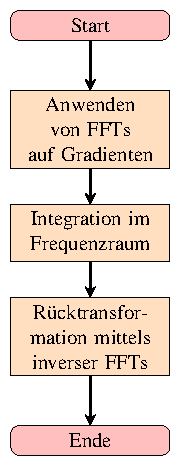
\includegraphics[width=0.17\linewidth]{pdf/graph_fc}}};
		\only<6>{\draw[red, very thick] (-4.3, -1.1) -- (-2, 2.5)};
		\only<6>{\draw[red, very thick] (-4.3, -1.8) -- (-2, -2.5)};
		\only<6>{\draw[red, very thick] (-2, -2.5) rectangle (0.0, 2.5)};
		
		\only<7>{\node at (0.5,1) {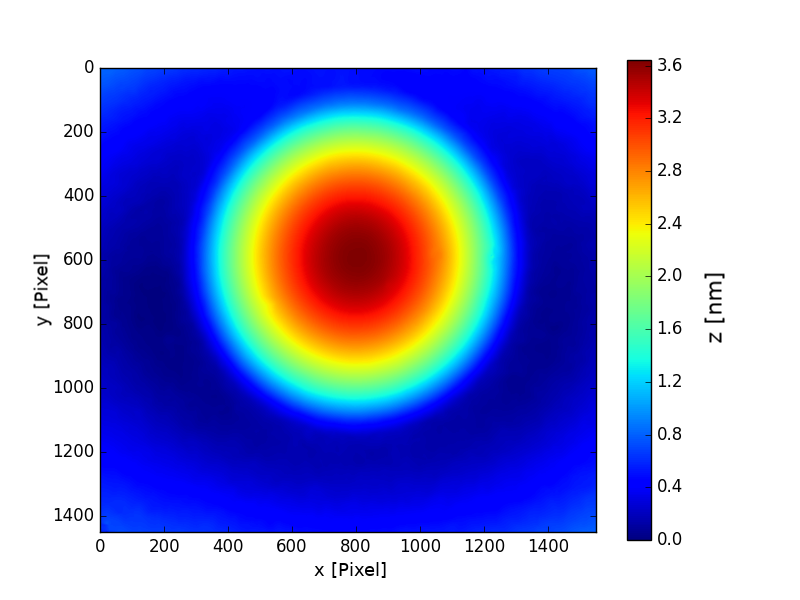
\includegraphics[width=0.6\linewidth]{img/2D_E10001_edf_ref_start0001_1-10_edf}}};
		\only<7>{\draw[red, very thick] (-2.7, -2) rectangle (3.4, 3.2)};
		\only<7>{\node at (0.7, -1.7) {Integrierte Gradientenmatrix}};
		\only<7>{\draw[red, very thick] (-4.3, -1.1) -- (-2.7, 3.2)};
		\only<7>{\draw[red, very thick] (-4.3, -1.8) -- (-2.7, -2)};
	\end{tikzpicture}
\end{frame}
\chapter{Performance-Analyse der derzeitigen Implementierung}

\section{Komplexität}

\subsection{Speckle-Tracking}

Der erste Schritt des Speckle-Trackings ist die Feststellung der starren Verschiebung. Werden hierfür feste Werte angenommen, ist diese Komplexität konstant. Wird allerdings ein Korrelationsverfahren verwendet, so ist die Komplexität $\mathcal{O}\left(\glssymbol{resolution} \cdot log\left(\glssymbol{resolution}\right)\right)$ für die \gls{resolution}, da hierfür \glspl{FFT} eingesetzt werden. 

Der nächste Verarbeitungsschritt ist der erste Durchlauf. Hier werden die Eingabebilder zunächst durch die Selektion der \gls{ROI}, also auf die \glsfirst{rroi} \glssymbol{rroi} verkleinert und anschließend in Blöcke mit konstanter Größe aufgeteilt, welche dann ineinander mittels des Template-Matchings gesucht werden. Die Komplexität der einzelnen Suchvorgänge kann somit auch als konstant angesehen werden. Der Durchlauf braucht demzufolge $\mathcal{O}\left(\gls{rroi}\right)$ Schritte. Die anschließende Interpolation wird auf alle Pixel des Bildes angewandt und hat demzufolge eine Komplexität von $\mathcal{O}\left(\gls{rroi}\right)$.

Der zweite Durchlauf, der als nächstes folgt, werden Subbilder, wie \ref{sec:speckle-tracking} beschrieben, generiert. durch die \glsfirst{uap} \glssymbol{uap} wird \gls{rroi}, und damit auch die Komplexität dieses Teils, mit dem Faktor $\gls{uap}^2$ verringert. Die \glsfirst{corrsize} \glssymbol{corrsize} legt nimmt auf das Template-Matching Einfluss, dessen Komplexität nun bei $\mathcal{O}\left(\gls{corrsize} \cdot log\left(\gls{corrsize}\right)\right)$ liegt. Der Einfluss der \glsfirst{gridResol} \glssymbol{gridResol} ist, ähnlich zu \gls{uap}, eine Verringerung mit dem Faktor $\gls{gridResol}^2$. Die Gesamtkomplexität der Template-Matchings im zweiten Durchlauf liegt somit bei:

\begin{center}
	$\mathcal{O}\left(\frac{\gls{rroi} \cdot \gls{corrsize} \cdot log\left(\gls{corrsize}\right)}{\left(\gls{uap}^2 \cdot \gls{gridResol}\right)^2}\right)$
\end{center}

Für die auf den Template-Matching-Prozess folgende Subpixel-Interpolierung werden neun Pixel in der Umgebung des Maximums jedes Übereinstimmungsmatrix interpoliert, womit dieser Schritt folgende Komplexität aufweist:

\begin{center}
	$\mathcal{O}\left(\frac{\gls{rroi}}{\left(\gls{uap}^2 \cdot \gls{gridResol}^2\right)}\right)$
\end{center}

Am Ende des Speckle-Tracking-Algorithmus wird versucht, nicht zuordenbare Ergebnisse mit einer anderen \glsfirst{corrsize} \glssymbol{corrsize} erneut zuzuordnen. Im schlimmsten Fall wird der zweite Durchlauf für die Hälfte der Subbilder \gls{ncorr}-fach wiederholt, wobei \gls{ncorr} die \glsdesc{ncorr} repräsentiert. Bei höheren Fehlerraten über 50\% bricht das Programm. In der hier als Grundlage vorliegenden Implementierung ist $\gls{ncorr} = 6$.

Die Gesamtkomplexität des Speckle-Tracking-Algorithmus liegt damit in der Komplexitätsklasse:

\begin{center}
	$\mathcal{O}\left(\frac{\gls{rroi} \cdot \gls{corrsize} \cdot log\left(\gls{corrsize}\right)}{\left(\gls{uap}^2 \cdot \gls{gridResol}\right)^2}\right)$
\end{center}

\subsection{Integration der Gradienten}

Um eine effiziente Integration der Gradienten zu ermöglichen, beruht der von \citeauthor{FC88} vorgeschlagene Algorithmus auf der Integration im Frequenzraum. Hierzu werden zuerst die Gradientenbilder mittels \glspl{FFT} in diesen Raum transformiert, dort in linearer Komplexität integriert und zum Schluss wieder zurück transformiert. 
Aufgrund der Verwendung von \glspl{FFT} befindet sich dieser Algorithmus in der Komplexitätsklasse:

\begin{center}
	$\mathcal{O}\left(\gls{resolution} \cdot log\left(\gls{resolution}\right)\right)$
\end{center}

\subsection{Hauptroutine}

Die Hauptroutine beginnt mit einer trivialen Parameterinitialisierung, die als linear angenommen werden kann. Auf diese folgt die Hauptschleife, welche für die \gls{N_Paare} jeweils ein mal ausgeführt wird. Hierzu werden zuerst die Sensorbilder mittels der bei der Kalibrierung ermittelten Werte mit einer Komplexität von $\mathcal{O}\left(\gls{resolution}\right)$ korrigiert. Dies wird gefolgt vom Speckle-Tracking-Algorithmus und der Integration der Gradienten. Die höchste Komplexität hat hier der Template-Matching-Algorithmus, welcher damit die Komplexitätsklasse und somit auch der gesamten Hauptroutine festlegt auf:

\begin{center}
	$\mathcal{O}\left(\frac{\gls{N_Paare} \cdot\gls{rroi} \cdot \gls{corrsize} \cdot log\left(\gls{corrsize}\right)}{\left(\gls{uap}^2 \cdot \gls{gridResol}\right)^2}\right)$
\end{center}

Dies liegt insbesondere für kleine \gls{uap} und \gls{gridResol} in der Komplexitätsklasse:

\begin{center}
	$\mathcal{O}\left(\gls{N_Paare} \cdot\gls{rroi} \cdot \gls{corrsize} \cdot log\left(\gls{corrsize}\right)\right)$
\end{center}

\section{Benchmark}

\subsection{Testsystem und Laufzeitumstände}

\paragraph{Testsystem}

\begin{sloppypar}
Alle Benchmarks liefen auf den \textit{haswell}-Partition des Taurus-Supercomputers an der Technischen Universität Dresden. Jeder Knote dieser Partition ist ausgestattet mit zwei Intel\textregistered \mbox{Xeon\textregistered} E5-2680 v3 \glspl{CPU}. Diese haben zwölf Rechenkerne, die mit bis zu 2.50 \gls{GHz} getaktet sind. MultiThreading war hierbei nicht aktiviert. Die Knoten haben 64 \gls{GiB} (\textit{haswell64}), 128 \gls{GiB} (\textit{haswell128}) oder 256 \gls{GiB} (\textit{haswell256}) Arbeitsspeicher zur Verfügung. Zusätzlich ist pro Rechenknoten eine 128 \gls{GB} \gls{SSD} installiert. Es wurde unter anderem Python 2.7.11 mit numpy 1.10.1 und OpenCV 3.1.0 verwendet. Eine komplette Liste aller geladenen Module lässt sich auf dem GitHub-Repository dieses Projektes\footnote{\url{https://github.com/ComputationalRadiationPhysics/Wavefront-Sensor/blob/cb7fd24ea64ad0fef0af93ba0dfb9f04f6487382/doc/loaded_libs.txt}} finden.
\end{sloppypar}

\paragraph{Laufzeitumstände}

Jede Konfiguration, bestehend aus Datensatz und Kernanzahl, wurde nach vier Aufwärmiterationen fünf mal ausgeführt. Hierbei wurden jeweils die reinen Ausführungszeiten des gesamten Skripts und einzelner Funktionen erfasst. Aus allen vorliegenden Zeiten wurde \gls{IO}-Zeiten herausgerechnet. Die Laufzeit mit den entsprechenden Datensätzen wurde auf unterschiedlich vielen Kernen von eins bis 24 gemessen. Jeder Benchmark lief exklusiv auf einem Knoten. 

\paragraph{Datensätze}

Zur Leistungsfeststellung der vorliegenden Implementierung werden drei verschiedene Arten von Datensätzen verwendet: \textit{detectorDistortion}, \textit{Experiment 6}, \textit{Lenses}. \textit{detectorDistortion} wird zur Kalibrierung verwendet. Die Eigenschaften dieser Typen werden in Tabelle \ref{tab:datasets} gegenüber gestellt.  Von diesem Datensatztyp gibt es einen Datensatz mit 25 Bildern. Es existieren drei \textit{Experiment 6} Datensätze mit 21 (\textit{Experiment 6 Lenses 200}), 11 (\textit{Experiment 6 Lenses 500}) und 14 Bildpaaren (\textit{Experiment 6 Lenses 1500}). Vom letzten Typ existieren vier Datensätze mit jeweils zehn (\textit{Lenses Set 1}), fünf (\textit{Lenses Set 2}), zwei (\textit{Lenses Set 3}) und einem Bildpaar.

\begin{table}
	\begin{tabularx}{\textwidth}{| X || X | X |}
		\hline
		& \multicolumn{2}{c|}{\textbf{Hauptroutine}} \\
		\cline{1-3}
		& Experiment 6 & Lenses \\
		\hline
		\hline
		\gls{rroi} (in Pixel) & Sensor 1: 550 x 550 \newline
		Sensor 2:1450 x 1450  & 1450 x 1550 \\
		\hline
		\gls{gridResol} & 1 & 1 \\
		\hline
		\gls{corrsize} & 91 & 41 \\
		\hline
		\gls{uap} & 1 & 1 \\
		\hline
		Pixelgröße & unterschiedlich & gleich \\
		\hline
	\end{tabularx}
	\caption{Parameter der Datensätze}
	\label{tab:datasets}
\end{table}

\subsection{Laufzeiten}

Die Laufzeiten der Konfigurationen, dargestellt in Abbildung \ref{fig:gesamtlaufzeiten}, variieren untereinander stark und reichen von ca. dreieinhalb Stunden für den \textit{Lenses Set 1}-Datensatz auf einem Kern bis hin zu ca. vier Minuten für den \textit{Lenses Set 3} Datensatz mit einem Bild auf 24 Kernen. Die Messpunkte sind hierbei dick hervorgehoben und die Skala ist logarithmisch eingeteilt. 

\begin{center}
	\begin{figure}
		\begin{subfigure}[b]{0.49\textwidth}
			\centering
			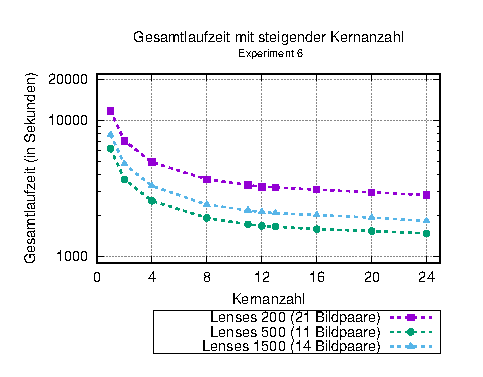
\includegraphics[width=\textwidth]{pdf/times_exp6}
			\caption[Experiment 6]{Experiment 6}
			\label{fig:times_exp6}
		\end{subfigure}
		\hfill
		\begin{subfigure}[b]{0.49\textwidth}
			\centering
			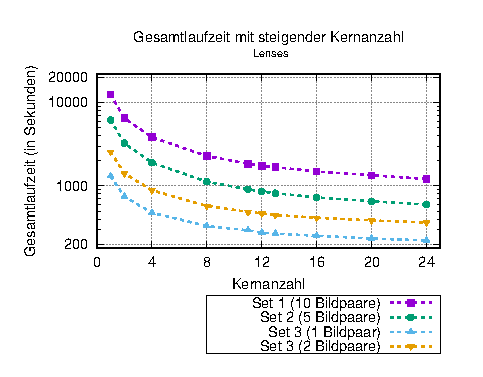
\includegraphics[width=\textwidth]{pdf/times_lenses}
			\caption[Lenses]{Lenses}
			\label{fig:times_lenses}
		\end{subfigure}
		\caption{Gesamtlaufzeiten}
		\label{fig:gesamtlaufzeiten}
	\end{figure}
\end{center}

Der Speedup des Programmes skaliert mit der Anzahl der Prozessorkerne nicht linear und flacht schnell ab. Der Speedup-Faktor für den \textit{Experiment 6} Datensätze übersteigt fünf nicht. Bei den \textit{Lenses}-Da\-ten\-sä\-tzen hingegen wird bei 24 Kernen ein Speedup von mehr als zehn erreicht. In den auf Abbildung \ref{fig:speedup} visualisierten Graphen ist eine starke Skalierung deutlich erkennbar. 

\begin{center}
	\begin{figure}
		\begin{subfigure}[b]{0.49\textwidth}
			\centering
			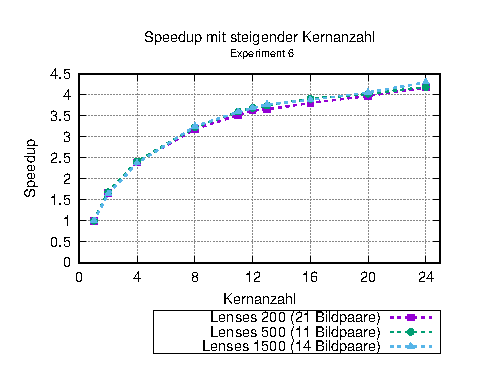
\includegraphics[width=\textwidth]{pdf/speedup_exp6}
			\caption[Experiment 6]{Experiment 6}
			\label{fig:speedup_exp6}
		\end{subfigure}
		\hfill
		\begin{subfigure}[b]{0.49\textwidth}
			\centering
			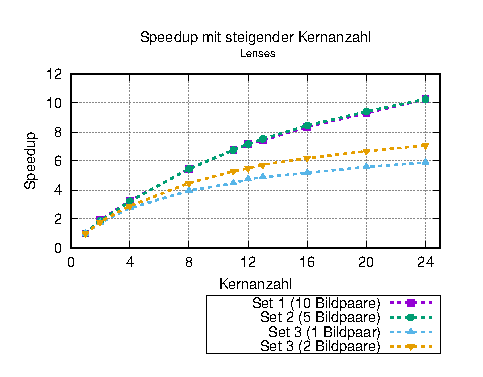
\includegraphics[width=\textwidth]{pdf/speedup_lenses}
			\caption[Lenses]{Lenses}
			\label{fig:speedup_lenses}
		\end{subfigure}
		\caption{Speedup}
		\label{fig:speedup}
	\end{figure}
\end{center}

Um Engpässe und besonders rechenaufwendige Funktionen zu identifizieren, wurde das Programm mit Zeitmessern versehen, die Ausführungszeiten und Aufrufanzahl protokolliert haben. Anschließend wurden es auf einem Rechenkern unter denselben Bedingungen, wie die anderen Konfigurationen, die Zeiten gemessen. Ein Überblick über das Gesamtprogramm mit seinen Subroutinen und deren Anteil an der Gesamtlaufzeit ist in Abbildung \ref{fig:perc_main} zu sehen.

\begin{center}
	\begin{figure}[htbp]
		\centering
		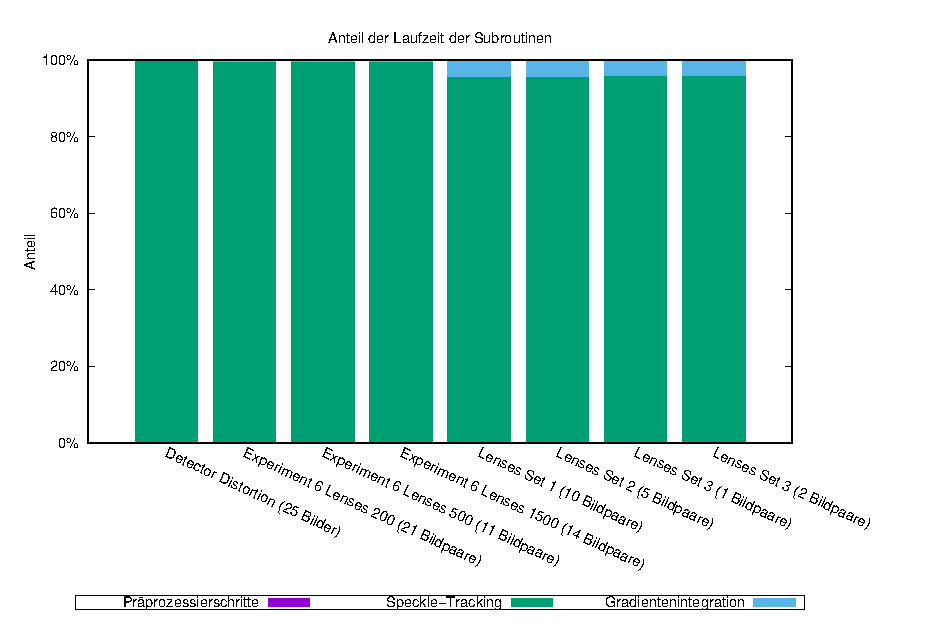
\includegraphics[width=0.7\textwidth]{pdf/main}
		\caption{Anteile der Laufzeiten}
		\label{fig:perc_main}
	\end{figure}
\end{center}

Hierbei ist eindeutig zu sehen, dass die meiste Zeit für das Speckle-Tracking benötigt wird. um weitere Informationen über die Laufzeiten der einzelnen Speckle-Tracking-Schritte zu gewinnen, wurde dieses ebenfalls mit Zeitmessern versehen. Die zeitliche Aufteilung dieser zeigt in Abbildung \ref{fig:perc_speckle}, dass hierbei der zweite Durchlauf am meisten Zeit benötigt. 

\begin{center}
	\begin{figure}[htbp]
		\centering
		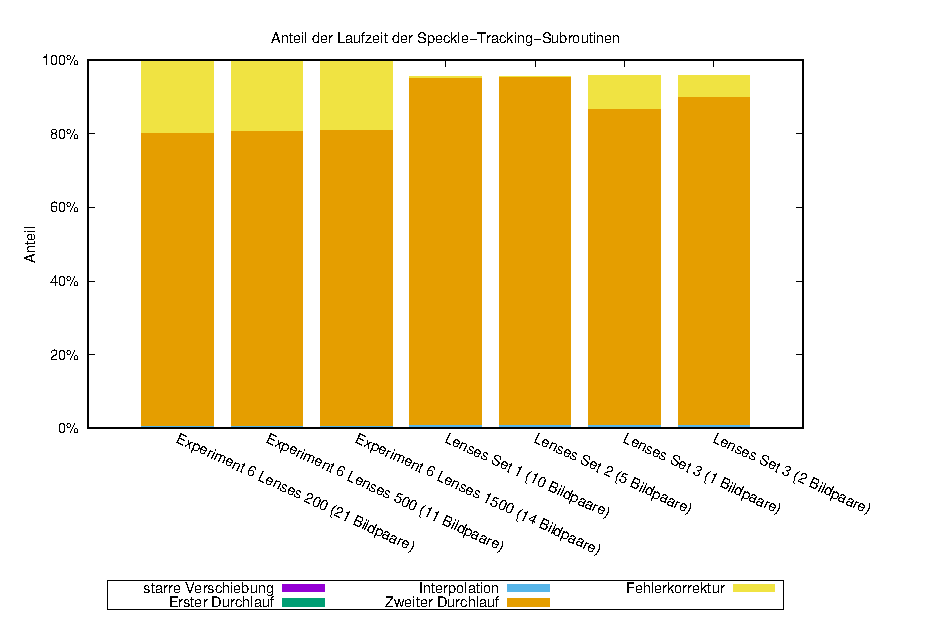
\includegraphics[width=0.7\textwidth]{pdf/speckle}
		\caption{Anteile der Laufzeiten des Speckle-Tracking-Algorithmus}
		\label{fig:perc_speckle}
	\end{figure}
\end{center}

Die kumulative Zeit der fünf rechenaufwendigsten Funktionen aller Konfigurationen, dargestellt in Abbildung \ref{fig:perc_slow}, liegt jeweils bei über 95\% der Gesamtzeit. 

\begin{center}
	\begin{figure}[htbp]
		\centering
		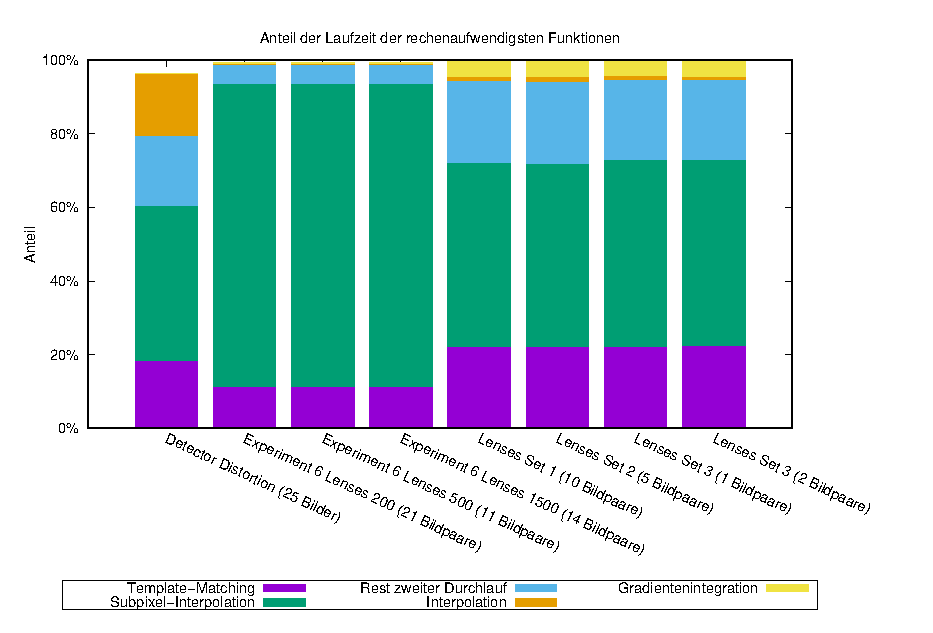
\includegraphics[width=0.7\textwidth]{pdf/slow}
		\caption{Anteile der Laufzeiten der langsamsten Funktionen}
		\label{fig:perc_slow}
	\end{figure}
\end{center}

\section{Grund der Performance-Engpässe}

Der Grund der langen Rechenzeiten des Template-Matchings und der Subpixel-Interpolation liegt in der hohen Anzahl der Aufrufe dieser begründet. Der zweite Durchlauf allein wird im \textit{Experiment 6 Lenses 200}-Datensatz über 5.3 Millionen mal aufgerufen. In jedem dieser Aufrufe wird das Template-Matching und die Subpixel-Interpolation jeweils ein mal genutzt. Hinzu kommt, dass, bis auf das Temp\-late-Match\-ing, der zweite Durchlauf nur geringen Gebrauch von bereits optimierten Bibliotheken wie numpy macht und somit der Pyhton-Overhead hinzukommt. 

Innerhalb des Speckle-Trackings ist der Aufruf des zweiten Durchlaufes mittels der joblib parallelisiert. Diese nutzt standardmäßig die multiprocessing-Bibliothek, welche für jeden Thread einen Fork der gesamten Python-Umgebung erstellen muss, was zu einem erheblichen Overhead führt\footnote{\url{https://pythonhosted.org/joblib/parallel.html}}.

Die hohe Rechenzeit der Gradienten-Integration ist im Aufruf dieser auf die Größe des Gesamtbildes begründet.

Insgesamt hat das Programm eine schlechte CPU-Auslastung von lediglich durchschnittlich 19,635\% \footnote{\url{https://github.com/ComputationalRadiationPhysics/Wavefront-Sensor/blob/f2fc5c2e5f8b4ef0e9b3ca3a4e770db67f230588/doc/cpu_util.md}}, wodurch häufig einige Kerne nicht oder nur wenig genutzt werden. 
\chapter{Parallelisierung der kritischen Abschnitte}

Um der optimalen Leistung nah zu kommen wurde bei der Implementierung ein iterativer Ansatz gewählt. Hierzu wurden zuerst die Möglichkeiten der Parallelisierung und anschließend die, der Optimierung in Python betrachtet. 

\section{Parallelisierung}

\subsection{Parallelisierung der Verarbeitung einzelner Bildpaare mittels MPI}

Da die zu bearbeitenden Bildpaare voneinander unabhängig sind, lassen diese sich trivial parallelisieren. Der Vorteil dieses Ansatzes liegt besonders in seiner simplen Implementierung und erwarteten linearen Skalierung begründet. Dieser Ansatz bringt allerdings auch einige Nachteile mit sich: Viele \gls{MPI}-Implementierungen erlauben keine neuen \correctme{Threads Nachweiß einfügen} und es ist nur eine schwache Skalierung zu erwarten. Sofern kein Multithreading innerhalb von \gls{MPI} möglich ist, limitiert die Anzahl der Bildpaare die Parallelisierungsmöglichkeiten stark, weshalb hier aus Zeitgründen auf intensives Testen dieser Version verzichtet wird. 

\subsection{Parallelisierung innerhalb der Verarbeitung einzelner Bildpaare mittels MPI}

Eine sinnvolle Erweiterung zur oben beschriebenen Methode ist das Ersetzen der genutzten Multithreading-Bibliothek mittels MPI, sodass selbst die Berechnung eines einzelnen Bildpaares über Rechnergrenzen hinweg möglich ist. In diesem Zuge wurde auch die Fehlerkorrektur am Ende des Speckle-Trackings parallelisiert, indem die zu korrigierende Bildausschnitte auf mehrere Kerne verteilt wurden. Zusätzlich ermöglicht diese Implementierung den Einsatz eines Tracing-Programmes, wie SCORE-P\footnote{\url{http://www.vi-hps.org/projects/score-p/}}. Dies war aufgrund der unterliegenden multiprocessing-Bibliothek zuvor nicht möglich. Ein hoher Speedup wird insbesondere für wenige zu korrigierende Bildausschnitte nicht erwartet. 

Im konkreten werden die Bildpaare auch \gls{CPU}-Kern Gruppen verteilt. Einer dieser Kerne agiert hierbei als Hauptkern und ist dafür verantwortlich das Bildpaar zu verarbeiten, wobei dieser Aufgaben mittels eines \gls{MPI}-Kommunikators an die anderen Rechenkerne verteilen kann. Dies ist in der Abbildung \correctme{Abbildung einfügen} gezeigt. Die Schnittstelle wurde hierbei ähnlich zur joblib-Implementierung entworfen. Sollten mehr Bildpaare als Rechenkerne vorhanden sein, werde mehrere Bildpaare von eine Kern hintereinander verarbeitet. Die Programmierschnittstelle wurde so entworfen, dass die Verteilung der Bildpaare auf die Kernen und das Parallelisieren innerhalb dieser für den Programmierer transparent geschieht. \correctme{Implementierung verlinken}

\correctme{\textbf{Schemata einfügen}}

\section{Optimierung der Python-Engpässe}

\begin{correctmore}
	- Optimieren einzelner in Python implementierter Programmteile, die sich als besonders langsam herausgestellt haben
\end{correctmore}

\subsection{Nutzen von bereits optimierter Funktionen}

Einige Teile des Codes können durch bereits in Python oder einer optimierten Bibliothek enthaltenen Funktion ersetzt werden, womit der Interpretieraufwand erheblich reduziert wird. Dies gehört damit zu einer der grundlegenden Optimierungsmöglichkeiten. Zusätzlich dazu sind diese Funktionen meist bereits für optimale Leistung optimiert. In der Funktion \textit{nxcorr\_disp} lassen sich solche Code-Abschnitte finden. Die Code-Auflistung \correctme{Auflistung referenzieren} zeigt die Implementierung in reinem Python und die Auflistung \correctme{Auflistung referenzieren} zeigt die Nutzung von bereits optimierten Funktionen. 

\begin{lstlisting}
for i in range(1,lengthY-1):
	for j in range(1,lengthX-1):
		if (nxcorr[i, j] > maxValue):
			maxValue = nxcorr[i, j]
			maxI = i
			maxJ = j
\end{lstlisting}

\begin{lstlisting}
nxcorr_small = nxcorr[1:-1,1:-1]
(_, maxValue, _, (maxJ, maxI)) = cv2.minMaxLoc(nxcorr_small)
maxI += 1
maxJ += 1
\end{lstlisting}

Des weiteren befindet sich in der \textit{nxcorr\_disp}-Funktion die Berechnung des Signal-Rausch-Verhältnisses (gezeigt in Auflistung \correctme{Auflistung referenzieren}), was allerdings im weiteren Verlauf des Programmes nicht wieder verwendet wird. 

\begin{lstlisting}
avg = 0.0
count = 0
for i in range(lengthY):
	for j in range(lengthX):
		if ((i is not maxI) and (j is not maxJ)):
			avg = avg + abs(nxcorr[i,j])
			count = count + 1
avg = avg / float(count)
SNr = maxValue / avg
\end{lstlisting}

Nachdem diesen Änderungen befindet sich keine in Python implementierte Schleife mehr in der Funktion. Angesichts der hohen Aufrufzahl der \textit{nxcorr\_disp} und dem Entfernen großer Codeanteile ist ein hoher Beschleunigungsfaktor zu erwarten. \correctme{Implementierung verlinken}

\subsection{Kompilieren}

Eine weitere Möglichkeit der Minimierung des Python-Engpasses ist die Übersetzung des Codes in nativen Maschinencode. Die möglichen Ansätze hierbei reichen von der Übersetzung des gesamten Programmes über die Übersetzung einzelner Funktionen, die in Python dann als Modul geladen werden können, bis hin zur Nutzung eines just-in-time Compilers, welcher annotierte Funktionen bei dessen ersten Aufruf in nativen Maschinencode übersetzt. 

\subsubsection{Gesamtes Programm}

\begin{correctmore}
	- kompilieren des kompletten Projektes mit Cython
	- funktioniert, aber Ergebnisse bringen nicht gewünschten Speedup bzw. nur manchmal
	--> Ansatz verworfen
\end{correctmore}

\subsubsection{Einzelne Funktionen}

\correctme{ - kompilieren einzelne Funktion}

\paragraph{numba}

\correctme{ - just in time compiler}

\paragraph{Cython}

\begin{correctmore}
	- regulärer Compiler
	- weitere Optimierungsmöglichkeiten (z.B. mit C Typen)
\end{correctmore}
\chapter{Performance-Messungen der parallelen Implementation}

Für die in diesem Kapitel durchgeführten Performance-Messungen wurde dasselbe Testsystem genutzt wie auch in Sektion \ref{sec:performance-messungen} beschrieben wurde. Die einzige Änderung hierbei ist, dass in vielen Benchmarks mehr als ein Knoten beansprucht wurde. Auch die Datensätze und die geladenen Module haben sich nicht geändert. Wie auch bei der Performance-Analyse, sind aus allen in diesem Kapitel angegeben Zeiten die \gls{IO}-Zeiten herausgerechnet worden. Ebenfalls wurde hier auch wieder nach vier Aufwärmiterationen für fünf Iterationen des Programmes die Zeit gemessen. 

\section{Evaluierung der Optimierungen}

\subsection{Parallelisierung}

Auf der Abbildung \ref{fig:mpi_speedup} ist für die auf dem GitHub-Branch \textit{mpi} verfügbare Version \cite{CBS18} deutlich ein Beschleunigungsfaktor von ca. zwei bis vier gegenüber der vorgegebenen Implementierung erkennbar. Anzumerken ist hierbei, dass als Referenz für den Speed-Up die Laufzeit der vorgegebenen Implementierung auf einem Kern genutzt wurde. Ebenfalls wird ersichtlich, dass diese Lösung nur mit der Anzahl der Eingabebildpaare skaliert, weshalb nur die \textit{Experiment 6 Lenses 200} und \textit{Lenses 500} mit 24 Kernen schneller ist als mit zwölf. Wie in Abbildung \ref{fig:mpi_times} zu sehen ist, liegen alle Laufzeiten dieser Version unter 1.000 Sekunden. Auch hier sind die Messpunkte wieder dick hervorgehoben und die Skala der Gesamtzeitgraphen ist logarithmisch eingeteilt. Ein Rechenknoten besitzt 24 Kerne, wodurch die Einteilung der X-Achse die Grenze der Rechenknoten verdeutlicht. 

\begin{center}
	\begin{figure}[h]
		\begin{subfigure}[b]{0.45\textwidth}
			\centering
			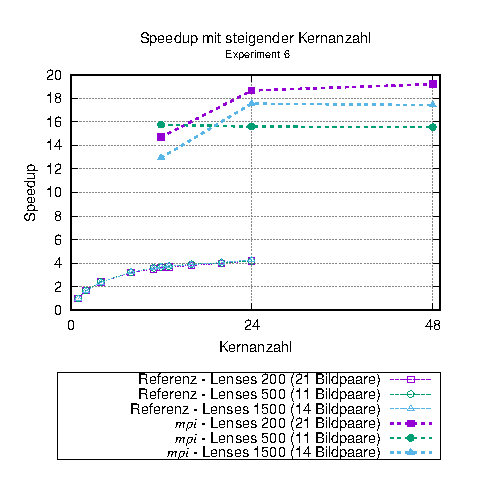
\includegraphics[width=\textwidth]{pdf/mpi_speedup_exp6}
			\caption{Experiment 6}
			\label{fig:mpi_speedup_exp6}
		\end{subfigure}
		\hfill
		\begin{subfigure}[b]{0.45\textwidth}
			\centering
			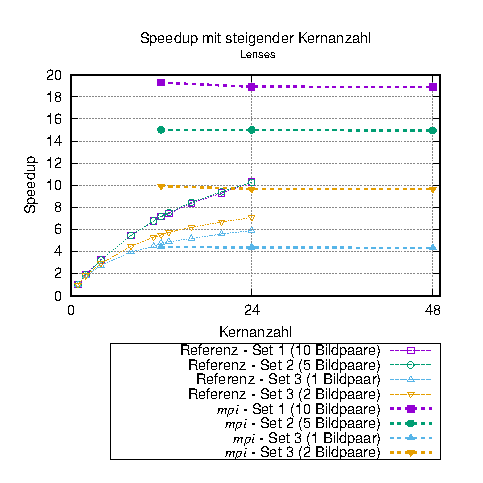
\includegraphics[width=\textwidth]{pdf/mpi_speedup_lenses}
			\caption{Lenses}
			\label{fig:mpi_speedup_lenses}
		\end{subfigure}
		\caption{Speed-Up der \textit{mpi} Implementierung gegenüber des von \citeauthor{Coj17} implementierten Python-Codes}
		\label{fig:mpi_speedup}
	\end{figure}
\end{center}

\begin{center}
	\begin{figure}[h]
		\begin{subfigure}[b]{0.45\textwidth}
			\centering
			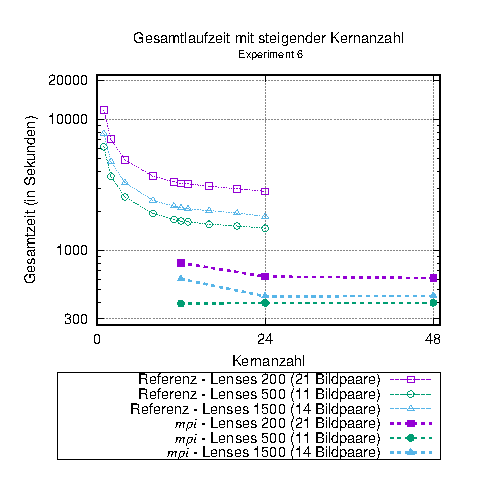
\includegraphics[width=\textwidth]{pdf/mpi_times_exp6}
			\caption{Experiment 6}
			\label{fig:mpi_times_exp6}
		\end{subfigure}
		\hfill
		\begin{subfigure}[b]{0.45\textwidth}
			\centering
			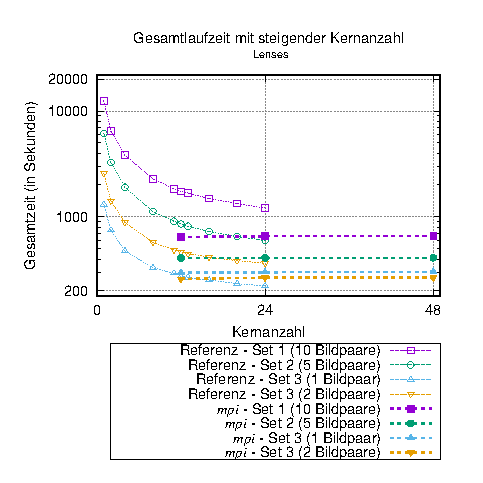
\includegraphics[width=\textwidth]{pdf/mpi_times_lenses}
			\caption{Lenses}
			\label{fig:mpi_times_lenses}
		\end{subfigure}
		\caption{Gesamtlaufzeit der \textit{mpi} Implementierung gegenüber des von \citeauthor{Coj17} implementierten Python-Codes}
		\label{fig:mpi_times}
	\end{figure}
\end{center}

Wie in Abbildung \ref{fig:mpi_advanced_speedup} zu sehen ist, schneidet die auf dem Branch \textit{mpi-advanced} verfügbare Version \cite{CBS18} für 24 Kerne schlechter ab als die \textit{mpi} Implementierung. Dies kann in der effizienteren Verteilung der Daten mittels der joblib-Bibliothek begründet liegen, da diese den in Linux effizient implementierten Fork-Befehl nutzt, wohingegen die \textit{mpi-advanced}-Implementierung die Daten direkt kopiert \cite{GVB+18}. Im Gegensatz zu der \textit{mpi}-Implementierung skaliert diese Version aber mit der Anzahl der verfügbaren \gls{CPU}-Kerne und nicht nur mit der Anzahl der Bildpaare. Anzumerken ist hier ebenfalls, dass die \textit{mpi}-Implementierung bei wenigen Kernen zwar schneller ist, aber deutlich mehr Arbeitsspeicher benötigt. Währenddessen die \textit{mpi-advanced}-Version unter Nutzung von 24 Kernen mit 64 \gls{GiB} auskommt, benötigt die \textit{mpi}-Version mehr als 128 \gls{GiB}.

Auch in der Abbildung \ref{fig:mpi_advanced_speedup} wurde wieder die auf einem Kern ausgeführte vorgegebene Implementierung als Referenz genutzt. 

\begin{center}
	\begin{figure}[h]
		\begin{subfigure}[b]{0.45\textwidth}
			\centering
			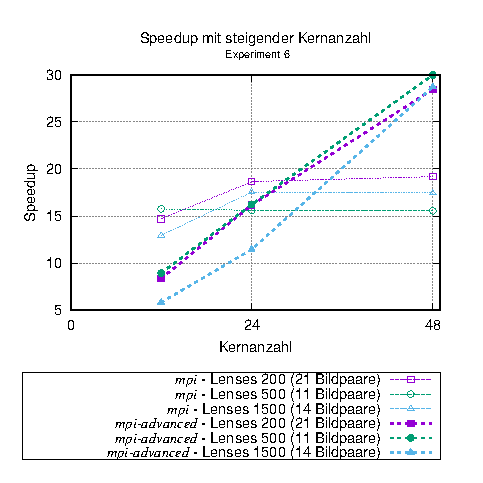
\includegraphics[width=\textwidth]{pdf/mpi_advanced_speedup_exp6}
			\caption{Experiment 6}
			\label{fig:mpi_advanced_speedup_exp6}
		\end{subfigure}
	\hfill
		\begin{subfigure}[b]{0.45\textwidth}
			\centering
			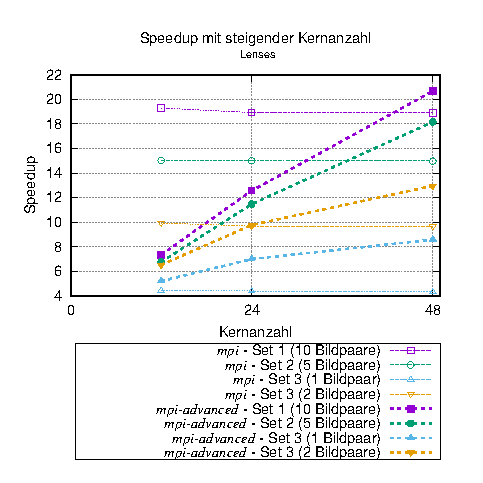
\includegraphics[width=\textwidth]{pdf/mpi_advanced_speedup_lenses}
			\caption{Lenses}
			\label{fig:mpi_advanced_speedup_lenses}
		\end{subfigure}
		\caption{Speed-Up der \textit{mpi-advanced} Implementierung gegenüber der \textit{mpi}-Version}
		\label{fig:mpi_advanced_speedup}
	\end{figure}
\end{center}

\begin{center}
	\begin{figure}[h]
		\begin{subfigure}[b]{0.45\textwidth}
			\centering
			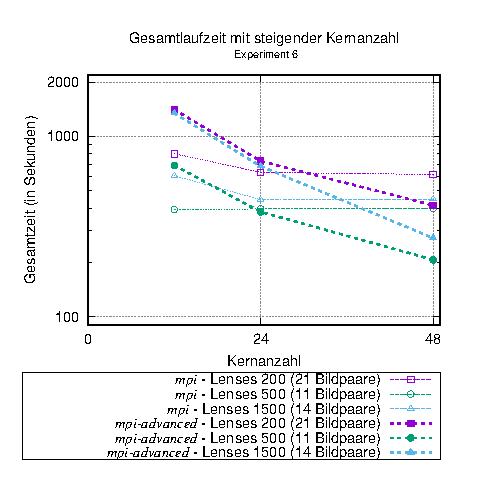
\includegraphics[width=\textwidth]{pdf/mpi_advanced_times_exp6}
			\caption{Experiment 6}
			\label{fig:mpi_advanced_times_exp6}
		\end{subfigure}
		\hfill
		\begin{subfigure}[b]{0.45\textwidth}
			\centering
			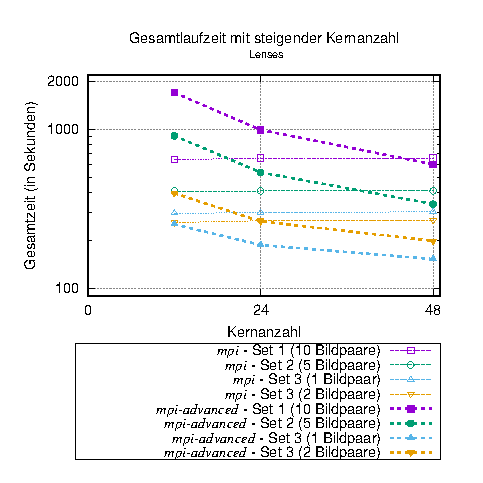
\includegraphics[width=\textwidth]{pdf/mpi_advanced_times_lenses}
			\caption{Lenses}
			\label{fig:mpi_advanced_times_lenses}
		\end{subfigure}
		\caption{Gesamtlaufzeit der \textit{advanced-mpi} Implementierung gegenüber des von Cojocaru implementierten Python-Codes}
		\label{fig:mpi_advanced_times}
	\end{figure}
\end{center}

\subsection{Optimierung von Python-Engpässen}

\subsubsection{Nutzen bereits optimierter Funktionen}

Wie in Abbildung \ref{fig:speedups_intrinsics} zu sehen ist, wurde mittels der Nutzung von bereits optimierten Funktionen ein Beschleunigungsfaktor von ca. vier für die \textit{Experiment 6}-Datensätze und ein Faktor zwischen 1,2 und 1,5 für die \textit{Lenses}-Datensätze erreicht. Der Speed-Up bei diesen Datensätzen war nicht so hoch, da diese weniger Bildpaare beinhalten und die Rechenzeit pro Bildpaar deutlich kleiner war, wodurch der Overhead durch das Senden der Daten einen größeren Einfluss auf die Gesamtlaufzeit hat. Die geringere Rechenzeit pro Bildpaar kommt durch die deutlich kleinere \gls{ROI}, eine kleinere \glsfirst{corrsize} \glssymbol{corrsize} und weniger zu korrigierenden Teilbilder zustande. Zusätzlich dazu entfällt die Notwendigkeit der Interpolation zwischen zwei verschiedenen Pixelgrößen, da hierfür nur ein Sensor im Einsatz war.

\begin{center}
	\begin{figure}[h]
		\begin{subfigure}[b]{0.54\textwidth}
			\centering
			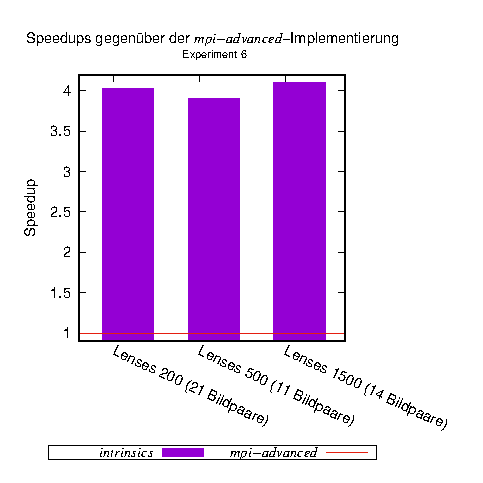
\includegraphics[width=\textwidth]{pdf/speedups_intrinsics_exp6}
			\caption{Experiment 6}
			\label{fig:speedups_intrinsics_exp6}
		\end{subfigure}
		\hspace{-0.9cm}
		\begin{subfigure}[b]{0.54\textwidth}
			\centering
			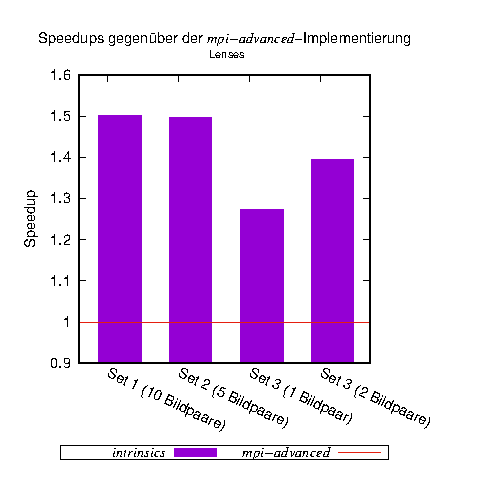
\includegraphics[width=\textwidth]{pdf/speedups_intrinsics_lenses}
			\caption{Lenses}
			\label{fig:speedups_intrinsics_lenses}
		\end{subfigure}
		\caption{Speed-Up der \textit{intrinsics} Implementierungen gegenüber der \textit{mpi-advanced}-Implementierung mit zwölf Kernen}
		\label{fig:speedups_intrinsics}
	\end{figure}
\end{center}

\begin{center}
	\begin{figure}[h]
		\begin{subfigure}[b]{0.54\textwidth}
			\centering
			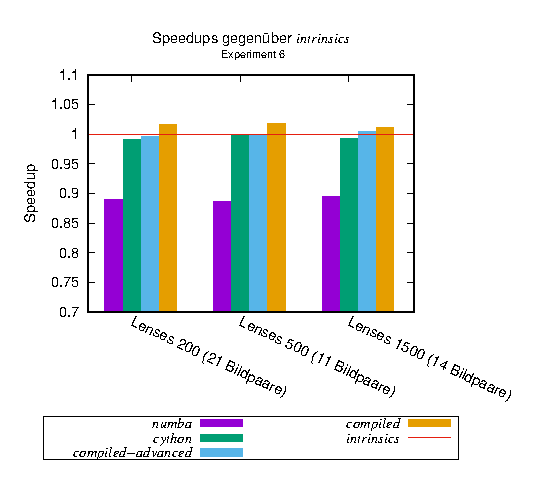
\includegraphics[width=\textwidth]{pdf/speedups_exp6}
			\caption{Experiment 6}
			\label{fig:speedups_exp6}
		\end{subfigure}
		\hspace{-0.9cm}
		\begin{subfigure}[b]{0.54\textwidth}
			\centering
			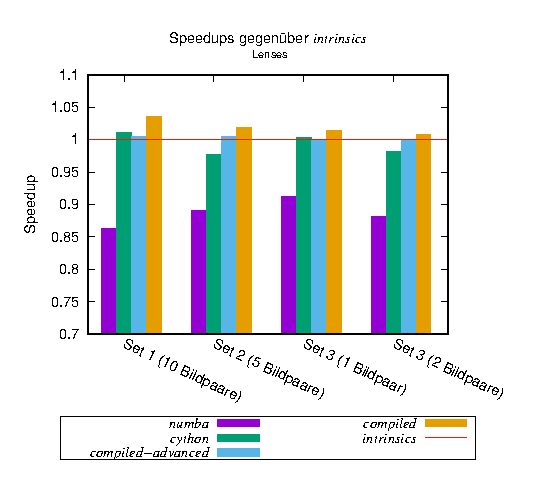
\includegraphics[width=\textwidth]{pdf/speedups_lenses}
			\caption{Lenses}
			\label{fig:speedups_lenses}
		\end{subfigure}
		\caption{Speed-Ups der einzelnen Implementierungen gegenüber der \textit{intrinsics} Implementierung mit zwölf Kernen}
		\label{fig:speedups}
	\end{figure}
\end{center}

\subsubsection{Kompilieren}

Die Abbildung \ref{fig:speedups} zeigt den Beschleunigungsfaktor der verschiedenen übersetzten Versionen gegenüber der Implementierung, welche bereits optimierte Funktionen nutzt. Hierbei ist deutlich ersichtlich, dass die Übersetzung des gesamten Programmes, welche auf dem \textit{compiled}-Branch verfügbar ist, immer schneller als die \textit{intrinsics}-Implementierung läuft. Der Grund für die höhere Leistung der \textit{compiled}-Implementierung ist hierbei nicht bekannt. Die \textit{numba}-Version hingegen schnitt immer deutlich schlechter als die anderen Versionen ab. Die Laufzeiten der \textit{cython}- und der \textit{compiled-advanced}-Versionen liegen nahe beieinander und bieten keinen Geschwindigkeitszuwachs gegenüber der \textit{intrinsics}-Implementierung. 

Die bereits gute Performance der \textit{intrinsics}-Implementierung liegt in der intensiven Nutzung optimierter Funktionen begründet, welche von einer Übersetzung der Python-Codes unberührt bleiben. Die Performance der \textit{numba}-Implementierung ist deutlich schlechter, da beim Aufruf einer \gls{JIT}-kompilierten Funktion diese erst in einer Liste aus übersetzten Funktionen gesucht werden muss, bevor diese aufgerufen werden kann \cite{PKA17}. Dieser Effekt wird dadurch verstärkt, dass die übersetzten Funktionen eine geringe Laufzeit haben, aber dafür sehr oft aufgerufen werden. Der zweite Durchlauf allein, und damit auch die \texttt{nxcorr\_disp()}-Funktion, wird im \textit{Experiment 6 Lenses 200}-Datensatz über 5.3 Millionen mal aufgerufen. 

\section{Skalierung}

Auf der Abbildung \ref{fig:best_speedup_standalone} ist eine lineare Skalierung gut erkennbar, bis die Anzahl der \gls{CPU}-Kerne die Anzahl der Bildpaare übersteigt. Anschließend stagniert der Beschleunigungsfaktor, da einige Bildpaare zwar mit mehr Kernen schneller bearbeitet werden können, aber das Programm auf die Fertigstellung der restlichen Bildpaare warten muss, die nur einen Kern zur Verfügung haben. Ein ähnliches Laufzeitverhalten lässt sich jedes Mal beobachten, wenn die Kernanzahl ein Vielfaches der Bildpaaranzahl erreicht. Da die Verarbeitung eines einzelnen Bildpaares nicht komplett parallelisiert werden kann, flacht laut Amdahl's Gesetz der Graph mit steigender Kernanzahl ab \cite{Amd67}. Die Gesamtlaufzeiten im Bezug auf die vorgegebene Implementierung ist in Abbildung \ref{fig:best_times} zu sehen. 

\begin{center}
	\begin{figure}[h]
		\begin{subfigure}[b]{0.45\textwidth}
			\centering
			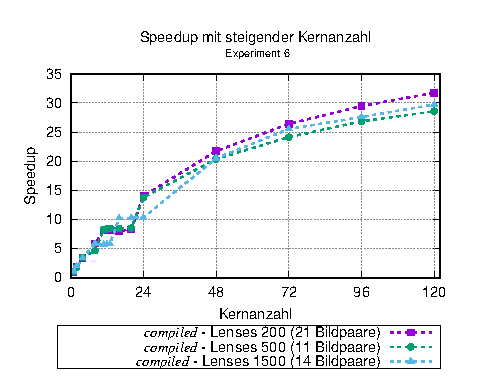
\includegraphics[width=\textwidth]{pdf/best_speedup_exp6_standalone}
			\caption{Experiment 6}
			\label{fig:best_speedup_exp6_standalone}
		\end{subfigure}
		\hfill
		\begin{subfigure}[b]{0.45\textwidth}
			\centering
			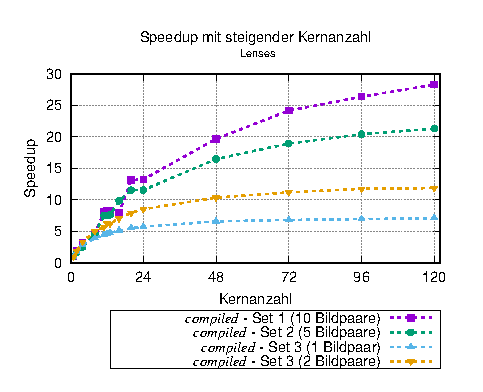
\includegraphics[width=\textwidth]{pdf/best_speedup_lenses_standalone}
			\caption{Lenses}
			\label{fig:best_speedup_lenses_standalone}
		\end{subfigure}
		\caption{Speed-Up der \textit{compiled} Implementierung}
		\label{fig:best_speedup_standalone}
	\end{figure}
\end{center}

\begin{center}
	\begin{figure}[h]
		\begin{subfigure}[b]{0.45\textwidth}
			\centering
			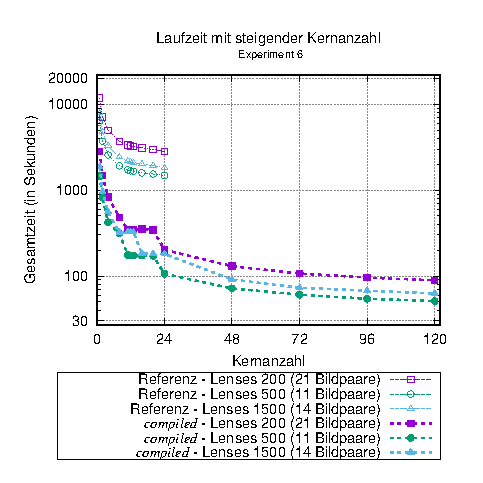
\includegraphics[width=\textwidth]{pdf/best_times_exp6}
			\caption{Experiment 6}
			\label{fig:best_times_exp6}
		\end{subfigure}
		\hfill
		\begin{subfigure}[b]{0.45\textwidth}
			\centering
			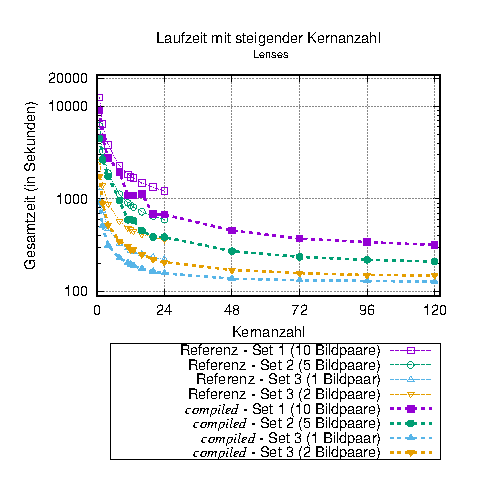
\includegraphics[width=\textwidth]{pdf/best_times_lenses}
			\caption{Lenses}
			\label{fig:best_times_lenses}
		\end{subfigure}
		\caption{Gesamtlaufzeit der \textit{compiled} Implementierung gegenüber des vorgegebenen Python-Codes}
		\label{fig:best_times}
	\end{figure}
\end{center}

Der Speed-Up-Graph in Abbildung \ref{fig:best_speedup_standalone} weist eine starke Skalierung auf, jedoch skaliert das Laufzeitverhalten schwach besser. Solang mehr Bildpaare als \gls{CPU}-Kerne an der Berechnung beteiligt sind, skaliert das Programm nahezu linear. Das Effizienzoptimum wird somit erreicht, wenn die Anzahl der \gls{CPU}-Kerne gleich der Anzahl der Bildpaare ist, da an diesem Punkt jeder Kern mit einem Bildpaar komplett ausgelastet ist und keine Zeit zum weiteren Verteilen der Daten aufgebracht werden muss. 

Eine Sättigung tritt bei allen Datensätzen ein, sobald mehr als 20 \gls{CPU}-Kerne pro Bildpaar eingesetzt werden. An diesem Punkt wird die meiste Rechenzeit in nicht parallelisierten Abschnitten des Speckle-Trackings und in der Gradientenintegration verbracht.
\chapter{Auswertung}

\section{Wertung des Ergebnisses}

Die Abbildung \ref{fig:best_speedup} zeigt einen deutlich erhöhten Speedup gegenüber der vorgegebenen Python-Implementierung. Für die \textit{Experiment 6}-Datensätze erreicht dieser einen Speedup von über 130 und für die \textit{Lenses}-Datensätze liegt der maximale Beschleunigungsfaktor bei bis zu 40 für den \textit{Set 1}-Datensatz. Bei der Wahl größerer Datensätze sind aufgrund mangelnder Parallelisierbarkeit der Bildpaare größere Beschleunigungsfaktoren zu erwarten.

\begin{center}
	\begin{figure}[htbp]
		\begin{subfigure}[b]{0.45\textwidth}
			\centering
			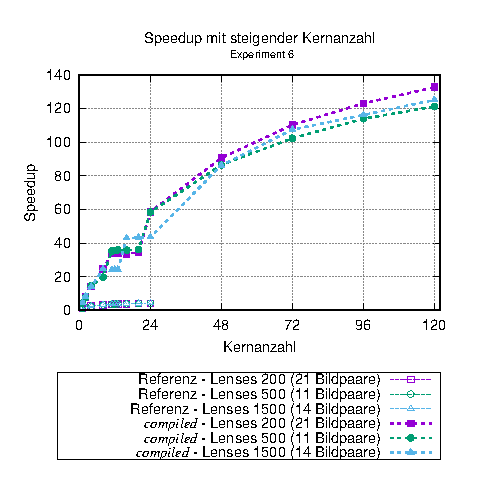
\includegraphics[width=\textwidth]{pdf/best_speedup_exp6}
			\caption{Experiment 6}
			\label{fig:best_speedup_exp6}
		\end{subfigure}
		\hfill
		\begin{subfigure}[b]{0.45\textwidth}
			\centering
			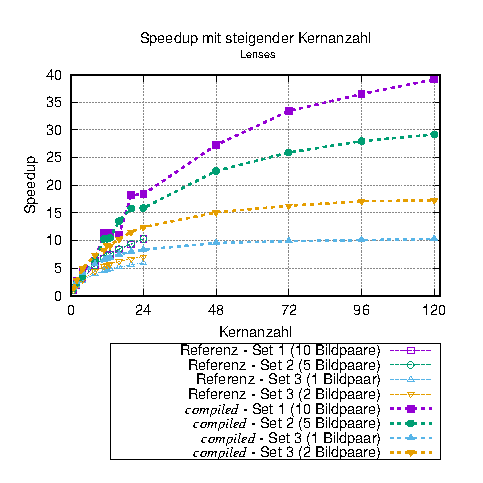
\includegraphics[width=\textwidth]{pdf/best_speedup_lenses}
			\caption{Lenses}
			\label{fig:best_speedup_lenses}
		\end{subfigure}
		\caption{Speedup der \textit{compiled} Implementierung gegenüber des von Cojocaru implementierten Python-Codes}
		\label{fig:best_speedup}
	\end{figure}
\end{center}

Trotz dessen, dass mit 120 \gls{CPU}-Kernen bereits ein Speedup von über 130 erreicht wurde, müsste die Anzahl der Bildpaare und der Kerne bei weitem höher sein, um die Echtzeitfähigkeit des Programmes sicher zu stellen. Dies ist in Größenordnungen von 2400 Bildpaaren und 2400 \gls{CPU}-Kernen zu erwarten, was bereits 100 Taurus-Knoten wären. 

\section{Verbesserungsmöglichkeiten}

Im Verlauf der Implementierung wurden viele der trivialsten Optimierungsmöglichkeiten implementiert. Während der letzten Iterationen der Implementierungen wurde allerdings auch weiteres Potential sichtbar. Beispielsweise ließe sich die Knoten interne Kommunikation mit Intrakommunikatoren oder geteiltem Speicher optimieren um den Kopieraufwand der Daten zu senken. 

Obwohl in dieser Arbeit bereits viele Optimierungen implementiert wurden und ein hoher Speedup erreicht wurde, gibt es immer noch weiteres Potential. Die Verwendung der FFTW\footnote{\url{http://www.fftw.org/}}-Bibliothek ist eine davon. Mithilfe dieser ist es möglich, die Gradientenintegration zu beschleunigen indem beim Start des Programmes sogenannte \textit{Wisdoms} erstellt werden, welche die Transformation eines Bildes in den Frequenzraum erheblich beschleunigen könnte. 

Des Weiteren ist es möglich für die am häufigsten aufgerufenen Funktionen Datenblöcke zu bilden und diese zu verarbeiten, sodass der Overhead der Funktionsaufrufe sinkt. Dies bildet ebenfalls eine gute Grundlage um diese Datenblockverarbeitung mittels numpy, numexpr oder numba weiter zu beschleunigen. Insbesondere kann hierbei auch die CUDA\footnote{\url{https://developer.nvidia.com/cuda-zone}} und OpenCL\footnote{\url{https://www.khronos.org/opencl}} Schnittstelle von numba genutzt werden, um Berechnungen mittels \glspl{GPGPU} auszulagern. 

Eine weitere Verbesserungsmöglichkeit liegt in einer Verbesserung des Belastungsausgleiches. Hierbei bestünde die Möglichkeit die Bildpaare in Packete zusammenzufassen und diese hintereinander auszuführen, sodass ein durchgängiger Betrieb möglich wäre. 

Auch Optimierungen am Algorithmus sind noch denkbar. Da aus dem Ergebnis des Template-Matchings nur die Position und der Wert des Maximums benötigt werden, ließe sich Bild und Template mit durch Skalierung verminderter Auflösung matchen. Hierbei entstandene Ungenauigkeiten können behoben werden, indem in der Region des Maximums ein genaueres Match durchgeführt wird. Da das Match mit reduzierter Auflösung eine Heuristik über die Maximal mögliche Übereinstimmung ist, kann anschließend in diesem der zweit höchste Wert betrachtet werden. Ist dieser größer als das Ergebnis des genauen Matches, besteht die Möglichkeit, dass dieses falsch ist und es kann auf den in der OpenCV-Bibliothek implementierten Template-Matching-Algorithmus zurückgreifen. Ist die Auflösung des Templates und des Bildes jedoch nicht durch ein und denselben Skalierungsfaktor teilbar, so kann die Skalierung auf eine niedrigere Auflösung bereits erhebliche Zeit in Anspruch nehmen. Hierzu ähnliche Optimierungsmöglichkeiten wurden bereits von Elena-Ruxandra Cojocaru implementiert (siehe \ref{sec:speckle-tracking}). 

Zu guter Letzt besteht auch noch die Möglichkeit der Optimierung des Kalibrierungsteiles des Programmes. 
\appendix
\section<presentation>*{\appendixname}
\subsection<presentation>*{Weiterführende Literatur}

\begin{frame}[allowframebreaks]
  \frametitle<presentation>{Weiterführende Literatur}
    
 	{\footnotesize
 		
  	\printbibliography}
  
\end{frame}

\end{document}
